% !TEX TS-program = xelatex
% !TEX encoding = UTF-8 Unicode

\providecommand{\home}{../..}
\documentclass[\home/main.tex]{subfiles}

\begin{document}

\chapter{Introduction}\label{ch:introduction}

\textbf{High-level problem statement to draw in the reader:}
Robotics promises to relieve humanity from repetitive tasks. Yet, why is there currently no robot that ties our shoelaces, weeds our gardens, and folds our shirts?
These tasks break the boundaries of the scripted environment for which existing robot technologies are programmed. Programmed robots follow routines to assemble cars and weld miniaturized electrical components at astounding speeds and fine-grained precision. However, these robots operate in a cage where every instruction is precisely defined with minimal room for deviation. Nevertheless, when robots are supervised by humans, they can operate outside their safety prisons. For example, the da Vinci\textregistered\ robot allows performing surgery by teleoperating robotic arms through a hand-operated console. However, there exist no adaptive cruise control for surgery yet.
Evidently, current robotic technologies contain an impressive repertoire of manipulation tasks solved within industrial or laboratory conditions.
Gracefully and productively adopting robots in our daily lives will significantly impact industry and society. Robots will sort and pack all types of objects in warehouses, install electrical wiring in our cars, helping elderly people dress, and clean up our houses.
\todo{Missen we hier het belang van dexterous manipulation niet?}
% VOORBEELDEN HIER als volgende zin
%     robot butler: is de was aan het plooien, voor oude mensen aan het zorgen, aan het opruimen, aan het koken 
%     industrie voorbeelden: sort and package objects, bake bread, clean-up the factory, replace eletrical wiring outside the international space station. 
%     probeer de voorbeelden zoveel mogelijk rond manipulatie te houden!


\textbf{Overgang Relevantie deformable objects.}
For the robot butler to become a reality, control algorithms need to loosen assumptions about the environment in which robots operate. Nowadays, robotic manipulation solutions require environments to be fully specified and the object's configuration to not change. However, the real world presents an infinite supply of configurations. To find solutions for this problem, we study the robotic manipulation of objects that provide an infinite amount of configurations: deformable objects.

% Endowing robots with skills to handle objects that deform on interaction helps to solve a general problem: how should the robot react if the configuration changes.

\section{Deformable object manipulation and robotic laundry}
% what is it 
Many everyday objects deform upon force interaction: the wires we use to charge our phones, the clothes we carry, and the sutures doctors use for stitching wounds.
% Robot laundry
\textbf{Hier kort over robotic laundry, het proces en waarom het moeilijk en interessant is. Eventueel economische cijfers toevoegen.}
% why is it relevant?
Folding clothing is not the typical tasks encountered in industry or robotics research that focuses primarily on grasping and manipulating rigid objects. Rigid objects do not deform during interaction and significantly reduce the required information. For example, grasping your morning coffee cup requires only knowing the position of the handle of the cup.
On the contrary, if the handle is highly deformable, you also need to reason about its shape and how it deforms depending on the planned manipulation.
Comprehending the challenges associated with planning for deformations can be done by understanding why modern robots and their control algorithms fail.
% However, modern pick-and-place robots already experience difficulties grasping rigid objects that are partially hidden or transparent. We first look at why modern robots and their control algorithms fail. 

\section{Traditional control pipelines do not work for folding cloth}
A daily-life example found in common kitchens illustrates the workings of today's industrial robots. Instead of manually slicing food into smaller pieces for cooking, one\todo{"one" of "you"?} can use a food processor to automate the slicing process.
%\footnote{In the Dutch language, a kitchen robot is unluckily used as a term for kitchen appliances that perform actuated whisk, mix and knead operations.}
. Using the food processor requires structuring the environment: one needs to equip the correct blade on the motor shaft, preprocess the food into a manageable size for the blade and feed it through the tube while activating the motor. Deviating from this setting can lead to minor failures and dangerous harm. For example, inserting oversized food slices might lead to motor stalling. More dangerously, there is no intelligence in consumer-grade appliances stopping the motor from turning the blades if you decide to insert your hand into the feeding tube.

Current robotic control pipelines are organized in a similar way as the given food processor example: structuring the environment and decomposing the problem. Decomposition of a large problem into subproblems is a general problem-solving and engineering paradigm that allows making assumptions that simplifies the solution strategy. In robotics, this modular approach is omnipresent and has led to incredible levels of automation and an increase in productivity \autocite{Graetz2018}. However, the innate fear that robots will soon take over our jobs \autocite{cave2019hopes} is unwarranted.
Open-loop control architectures with no adaptability towards deviations and failures elsewhere in the control pipeline will repeatedly fail when variations occur in the routine. Some of the most advanced robotics research and development teams demonstrate this in the 2015 DARPA Robotics Challenge Finals \autocite{DARPA2015}. The consequences of exposing robots to unstructured environments can be viewed in published video clips \autocite{darpaVideos}: million-dollar robots tumbling to the ground in, frankly, hilarious ways. In one example, a robot is supposedly turning a valve. However, the robot's walking path is misaligned, making it stand next to the valve instead in front of it. Consequently, the robot is performing a rotating movement with its arm in thin air while assuming resistance of the valve for balancing. The missing counterbalance makes the robot falls to the ground. The rotating valve failure brings the inner working of control loops to light: a sequence of isolated modules that solve decomposed tasks with no regard for failures down- or upstream in the pipeline.
% This is frappant considering with how much apparent ease humans solve similar tasks. 

Robots that manipulate deformable objects employ similar pipelines: a sequence of modules with functionalities ranging from garment type identification, to corner point detection and executing preprogrammed folding sequences. We visualize a canonical pipeline for folding clothing in \cref{fig:intro_canonical_control_pipeline}. These approaches are assumption-heavy and can have limited generalization. This motivates our research to look in the direction of employing machine learning based methods to train controllers that can perform robust grasp synthesis when faced with novel conditions.

\begin{figure}
    \centering
    \subfile{figures/fig-canonical-manipulation-pipeline-folding.tex}
    \caption{Canonical robotic control pipeline for folding clothing. Each module solves an isolated task and passes the result to the next module.}
    \label{fig:intro_canonical_control_pipeline}
\end{figure}

\section{From engineered pipelines to end-to-end learning}
Machine learning is a subset of \gls{AI} methods that are able to learn patterns from examples. The successes of deep neural networks, a machine learning method, in playing Atari video games \autocite{Mnih2015} and beating human champions in the game of Go \autocite{gaemofGo2016}, has driven researchers to adopt machine learning across the whole pipeline. This had led to an end-to-end learning approach in which a camera image, or other input, is given to the robot and has to actuate its motors based directly. Every functional module in the pipeline on the top in \cref{fig:intro_end2end}, for example, is replaced integrally with a deep neural network.

Unfortunately, end-to-end learning for robotics is priviliged to organisations containing massive computational power and expensive robotic farms.
deze robots worden dan in een RL framework geplaatst waar ze moeten interageren. Dit zou nog grappigere beelden oplveren dan DARPA 2015: robots dat zich niet bewust zijn van hun ledematen moeten hun motoren leren aansturen om bv kledij te vouwen. Imagine the situations. Although, most robots would probably fall down quickly and harm themselves in the process. 

Hence, in this research, we aim to democratise robotic learning by accelerating robotic learning. 

\begin{figure}[htpb]
    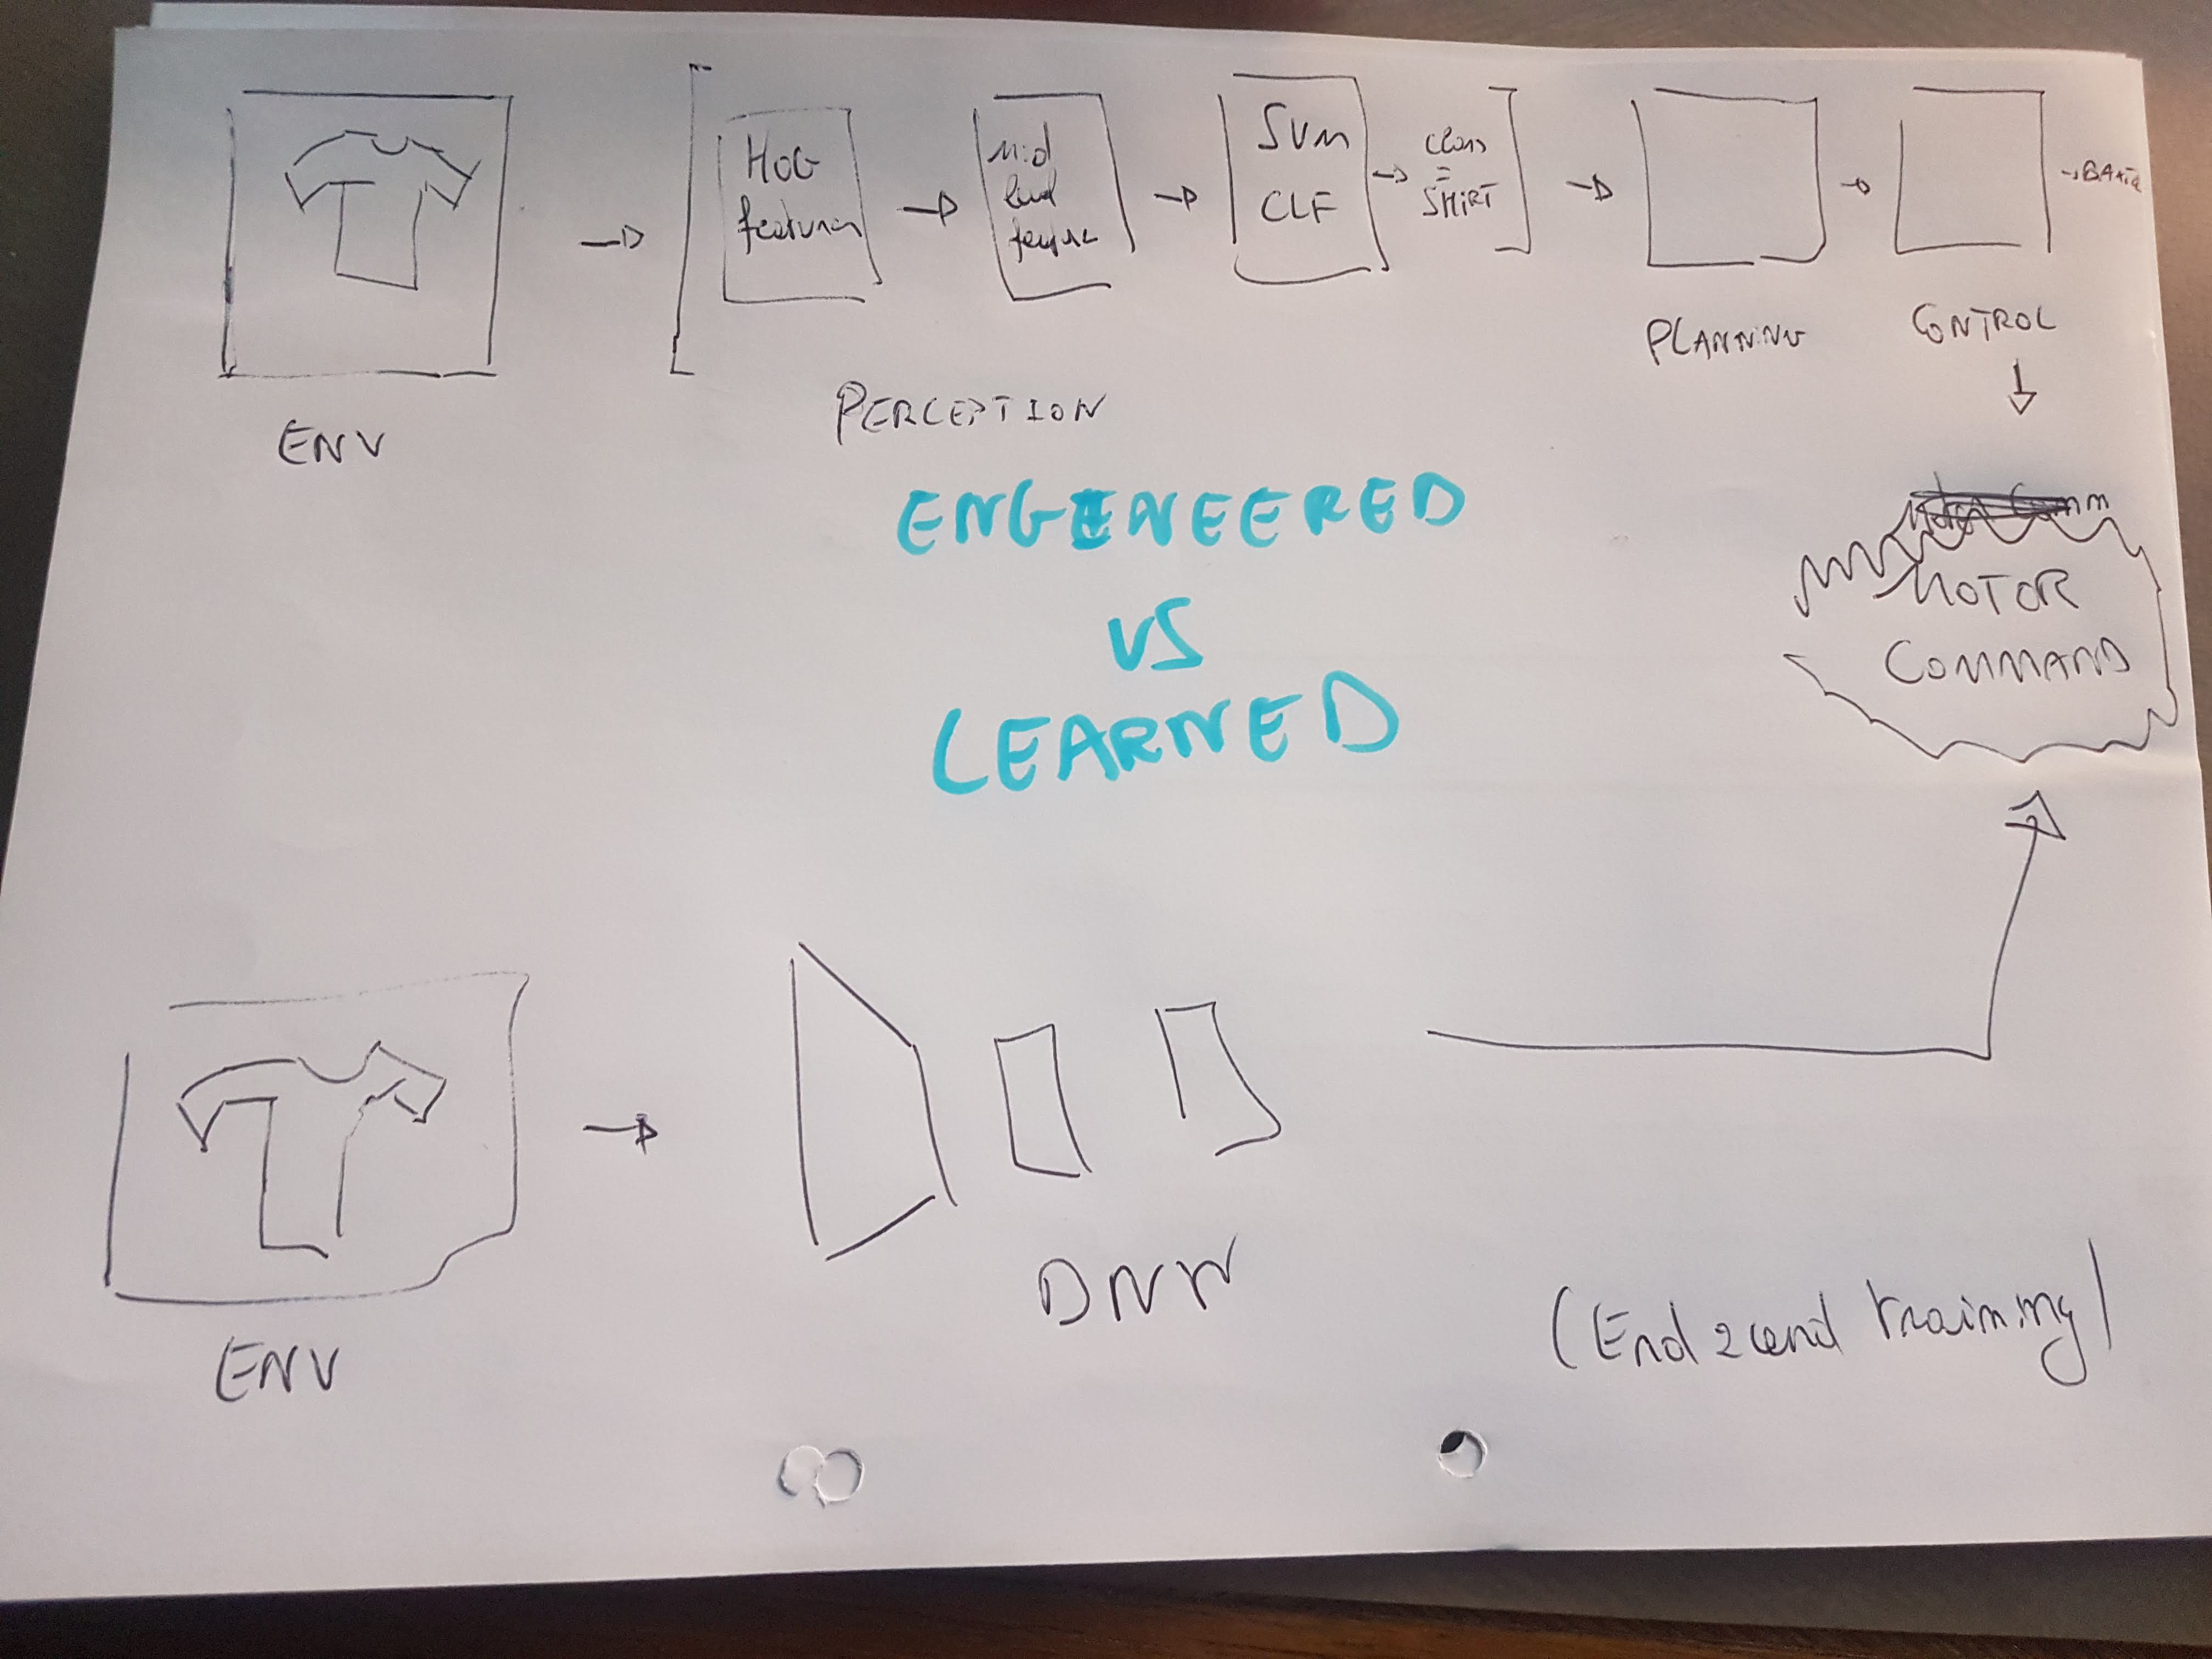
\includegraphics[width=\linewidth]{\home/chapters/01-introduction/figures/end2end-mockup}
    \caption{\textbf{Standard robotic control pipelines versus end-to-end architectures.} The diagram on the top shows how an image is processed to manually tuned features in order to do state estimation. This is then used downstream for trajectory planning and motor control. The diagram on the bottom shows an end-to-end approach to the same problem: an image is given to a deep neural network that learns its own features and executes actions directly on the actuators.}
    \label{fig:intro_end2end}
\end{figure}

TODO: eventueel wat inspiratie bij Seita halen? 

\section{Accelerating learning of robotic manipulation of deformable objects}

cfr miro board en bijhorende subsecties. Steeds luchtig naar formeel.


\subsection{Datasets}
\subsection{Simulation}
\subsection{Instrumentation}
When we use our hands to crush a plastic cup, multiple sensors of our body activates: we use our eyes to observe the deformations, our ears register the amplitude of the impact, our hands notify us of how much force we are applying and our proprioceptive system signal us how much crumbling there still can be done. This rich interplay of multiple modalities in the human cognitive system is in stark contrast to robotic manipulation pipelines that are largely vision-based.  Vision is important for robotic manipulation: it helps inferring the object location relative to the robot end-effectors, it helps understanding the objects geometry and some of its physical properties. Furthermore, commercial cameras are readily available and accessible compared to other sensors such as tactile sensors. Nevertheless, considering the giant leaps of object recognition using deep learning, robots still struggle recognizing objects in more difficult contexts such as partial occlusion, transparent object and moving objects \autocite{Guo2014,sajjan2019cleargrasp,Ojha2015}. 
Incorporating heterogenous sources of information can alleviate problems when state estimation cannot be directly observed from pixels. For example, finding the occluded corner of a crumbled towel is possible using sensing and simplifies the folding process considerably. 
We denote the process of adding sensory information to the learning environment of a robot as \textbf{instrumentation}. The goal is to direct the large focus on using vision-based state estimation to applying other sensor modalities in the environment such as tactile sensing in a cloth and force sensing in the fingers. Our hypothesis is that some modalities encode parts of the state in a much compacter way compared to vision. This semantic more meaningful encoding accelerates learning, which is important in robotics where real rollouts are expensive. 

\section{Research outline}
Our main goal is to investigate how learning-based approaches can be accelerated for . We focus exclusively on the application of robotic manipulation of cloth.

Simulation-driven approach
Dataset with people folding clothing
Low-cost robot setup to fold cloth in-vivo
Instrumentation
Unsupervised reward function

\section{Publications}

\end{document}
